% ---------- Titelblad Masterproef Faculteit Wetenschappen -----------
% Dit document is opgesteld voor compilatie met pdflatex.  Indien je
% wilt compileren met latex naar dvi/ps, dien je de figuren naar
% (e)ps-formaat om te zetten.
%                           -- december 2012
% -------------------------------------------------------------------
\RequirePackage{fix-cm}
\documentclass[12pt,a4paper,oneside]{book}

% --------------------- In te laden pakketten -----------------------
% Deze kan je eventueel toevoegen aan de pakketten die je al inlaadt
% als je dit titelblad integreert met de rest van thesis.
% -------------------------------------------------------------------
\usepackage{graphicx,xcolor,textpos}
\usepackage{helvet}
\usepackage{tikz}
\usetikzlibrary{fit,shapes,arrows,positioning,calc}
\usepackage{wrapfig}
\usepackage{chngcntr}
\usepackage{amsmath}
\usepackage{graphicx,caption}
\usepackage{subcaption}
\counterwithout{figure}{chapter}
\counterwithout{table}{chapter}
\newcommand\tab[1][1cm]{\hspace*{#1}}

\usepackage[acronym]{glossaries}
\newacronym{fcc}{FCC}{freely chosen cadence}
\newacronym{cvt}{CVT}{continu variabele transmissie}
\newacronym{dt}{DT}{decision tree}
\newacronym{rf}{RF}{random forest}
\newacronym{ma}{ms}{moving average}
\newacronym{es}{es}{exponential smoothing}
\newglossaryentry{r}{
  name = $r$ ,
  description = Input vector fietser,
}
\newglossaryentry{u_cy}{
  name = $u_{cy}$ ,
  description = Input vector fiets\,{} geleverd door de fietser,
}
\newglossaryentry{u_contr}{
  name = $u_{contr}$ ,
  description = Input vector fietser\,{} geleverd door de controller
}
\newglossaryentry{y}{
  name = $y$ ,
  description = Output vector fiets
}
\newglossaryentry{fcc_est}{
  name = $FCC_{est}$ ,
  description = Schatting van FCC\,{} geleverd door de cadanscontroller,
}
\newglossaryentry{v_ref}{
  name = $v_{ref}$ ,
  description = Referentie snelheid van de fietser,
}
\newglossaryentry{t_cy}{
  name = $T_{cy}$ ,
  description = Koppel geleverd door de fietser,
}
\newglossaryentry{t_cy,m}{
  name = $T_{cy,m}$ ,
  description = Gemeten koppel geleverd door de fietser,
}
\newglossaryentry{u_c}{
  name = $u_c$ ,
  description = Knop die bepaald of de cadans veranderd,
}
\newglossaryentry{theta_cr}{
  name = $\theta_{cr}$ ,
  description = Hoek van de trapas,
}
\newglossaryentry{v_bike}{
  name = $v_{bike}$ ,
  description = Snelheid van de fiets,
}
\newglossaryentry{helling}{
  name = $\alpha$ ,
  description = Helling,
}
\newglossaryentry{t_dc}{
  name = $T_{dc}$ ,
  description = Het DC koppel van de fietser (gemiddeld koppel),
}
\newglossaryentry{t_dc_max}{
  name = $T_{dc,max}$ ,
  description = Maximum DC koppel dat geleverd kan worden,
}
\newglossaryentry{omega_cr}{
  name = $\omega_{cr}$ ,
  description = Cadans in rpm,
}
\newglossaryentry{fcc_pred}{
  name = $FCC_{pred}$ ,
  description = Voorspelde FCC,
}
\newglossaryentry{k_cr,r}{
  name = $k_{cr,r}$ ,
  description = Verhouding overbrenging trapas-ringwiel,
}
\newglossaryentry{nr}{
  name = $nr$ ,
  description = Aantal tanden op het ringwiel,
}
\newglossaryentry{ns}{
  name = $ns$ ,
  description = Aantal tanden op het zonnewiel,
}
\newglossaryentry{s}{
  name = $S$ ,
  description = Ondersteuningsniveau,
}
\newglossaryentry{f_grav}{
  name = $f_{grav}$ ,
  description = Gravitationele last,
}
\newglossaryentry{f_friction}{
  name = $f_{friction}$ ,
  description = Wrijvings last,
}
\newglossaryentry{f_aero}{
  name = $f_{aero}$ ,
  description = Luchtweerstand,
}
\newglossaryentry{f_load}{
  name = $f_{load}$ ,
  description = Totale last,
}
\newglossaryentry{m}{
  name = $m$ ,
  description = Totaal gewicht van fiets en fietser,
}
\newglossaryentry{g}{
  name = $g$ ,
  description = Gravitationele constante,
}
\newglossaryentry{c_r}{
  name = $c_r$ ,
  description = Rolweerstand coëfficiënt,
}
\newglossaryentry{c_d}{
  name = $c_d$ ,
  description = Luchtweerstand coëfficiënt,
}
\newglossaryentry{rho_aero}{
  name = $\rho_{aero}$ ,
  description = Luchtdichtheid,
}
\newglossaryentry{a_aero}{
  name = $A_{aero}$ ,
  description = Frontaal oppervlak fietser,
}
\newglossaryentry{t_mg2}{
  name = $T_{MG2}$ ,
  description = Koppel geleverd door motor op het voorwiel,
}
\newglossaryentry{t_rw}{
  name = $T_{rw}$ ,
  description = Koppel op het achterwiel,
}
\newglossaryentry{r_w}{
  name = $r_w$ ,
  description = Straal van het voor- en achterwiel,
}
\newglossaryentry{p}{
  name = $P$ ,
  description = Vermogen,
}
\newglossaryentry{sf}{
  name = $sf$ ,
  description = Smoothing factor,
}
\newglossaryentry{f_k}{
  name = $f_k$ ,
  description = Factor voor fietsersmodel in functie van het gemiddeld koppel,
}
\newglossaryentry{f_h}{
  name = $f_k$ ,
  description = Factor voor fietsersmodel in functie van het gemiddeld koppel,
}
\newglossaryentry{f_v}{
  name = $f_k$ ,
  description = Factor voor fietsersmodel in functie van het gemiddeld koppel,
}
\newglossaryentry{k}{
  name = $K$ ,
  description = Agressiviteits parameter voor proportionele regelaar,
}

 
\makeglossaries


% -------------------- Pagina-instellingen --------------------------
% Indien je deze wijzigt, zal het titelblad ook wijzigen.  Dit dien je
% dan manueel aan te passen.
% --------------------------------------------------------------------

\topmargin -10mm
\textwidth 160truemm
\textheight 240truemm
\oddsidemargin 0mm
\evensidemargin 0mm

% ------------------- textpos-instellingen ---------------------------
% Enkele andere instellingen voor het voorblad.
% --------------------------------------------------------------------

\definecolor{green}{RGB}{172,196,0}
\definecolor{bluetitle}{RGB}{29,141,176}
\definecolor{blueaff}{RGB}{0,0,128}
\definecolor{blueline}{RGB}{82,189,236}
\setlength{\TPHorizModule}{1mm}
\setlength{\TPVertModule}{1mm}

\renewcommand{\contentsname}{Inhoudstafel}
\renewcommand{\listfigurename}{Lijst van figuren}
\renewcommand{\listoftables}{Lijst van tabellen}

\renewcommand{\chaptername}{Hoofdstuk}

\begin{document}

% ---------------------- Voorblad ------------------------------------
% Vergeet niet de tekst aan te passen:
% - Titel en, indien van toepassing, ondertitel
%          voor eventuele formules in de titel of ondertitel
%          gebruik je  \form{$...$}
% - Je naam
% - Je (co)promotor, begeleider (indien van toepassing)
% - Je opleiding
% - Het academiejaar
% --------------------------------------------------------------------
\thispagestyle{empty}
\newcommand{\form}[1]{\scalebox{1.087}{\boldmath{#1}}}
\sffamily
%
\begin{textblock}{191}(-24,-11)
\colorbox{green}{\hspace{113mm}\ \parbox[c][18truemm]{100mm}{\textcolor{white}{FACULTEIT COMPUTERWETENSCHAPPEN}}}
\end{textblock}
%
\begin{textblock}{70}(-18,-19)
\textblockcolour{}
\includegraphics*[height=19.8truemm]{LogoKULeuven}
\end{textblock}
%
\begin{textblock}{160}(-6,63)
\textblockcolour{}
\vspace{-\parskip}
\flushleft
\fontsize{40}{42}\selectfont \textcolor{bluetitle}{Real-Time Cadansaanpassing in een Automatische fietstransmissie }\\[1.5mm]
\end{textblock}
%

\begin{textblock}{160}(8,153)
\textblockcolour{}
\vspace{-\parskip}
\flushright
\fontsize{14}{16}\selectfont \textbf{Arno Cools}
\end{textblock}
%
\begin{textblock}{70}(-6,191)
\textblockcolour{}
\vspace{-\parskip}
\flushleft
Promotor:\\Prof. M. Moens\\[-2pt]
\vspace{5mm}
Begeleider:\\
\textsl{Ir. Tomas Keppens\\Ir. Jorrit Heidbuchel\\Ir. Rugen Heidbuchel}\\[-2pt]
\end{textblock}
%
\begin{textblock}{160}(8,191)
\textblockcolour{}
\vspace{-\parskip}
\flushright
Proefschrift ingediend tot het\\[4.5pt]
behalen van de graad van\\[4.5pt]
Master of Toegepase Informatica\\
\end{textblock}
%
\begin{textblock}{160}(8,232)
\textblockcolour{}
\vspace{-\parskip}
\flushright
Academiejaar 2018-2019
\end{textblock}
%
\begin{textblock}{191}(-24,248)
{\color{blueline}\rule{550pt}{5.5pt}}
\end{textblock}
%
\vfill
\newpage

% Als je het titelblad wil integreren met de rest van je thesis,
% kan je hieronder verder.
% ----------------------- Eerste pagina's -------------------------
% Hier kan je inhoudsopgave, voorwoord en dergelijke kwijt.
% -----------------------------------------------------------------
\rmfamily
\frontmatter
\pagenumbering{roman}
\setcounter{page}{0}
\chapter{Voorwoord}

A preface

\chapter{Abstract}

An abstract.
\tableofcontents
\listoffigures
\addcontentsline{toc}{chapter}{Lijst van figuren}

\chapter{Lijst van afkortingen en symbolen}
\printglossary[type=\acronymtype,title=Afkortingen]
\printglossary[title=Symbolen]

\mainmatter
\pagenumbering{arabic}

\chapter{Probleemstelling}
\section{Mobiliteitsvraagstuk}
De auto is het slachtoffer geworden van zijn eigen succes: we staan meer dan ooit in de file en de CO2 van personenverkeer stijgt jaar na jaar. De belg neemt al snel de auto voor korte afstanden ($<$ 25 km). In deze auto zit meestal maar 1 persoon. Het Belgische wagenpark blijft groeien (figuur \ref{fig:wagenpark}). Hier zien we wel een trend ontstaan. Er worden steeds meer elektrische en hybride wagens verkocht, maar die staan natuurlijk net zo goed in de file. Mobiliteit op twee wielen kan hier een oplossing bieden.
\\

\begin{wrapfigure}{R}{0.40\textwidth}
  \centering
  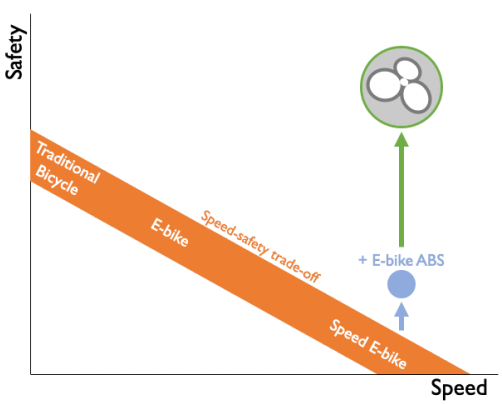
\includegraphics[width=1.1\linewidth]{images/snelheid-veiligheid-tradeoff.png}
  \caption{Snelheid-veiligheid trade-off (bron: IntuEdrive)}
  \label{fig:snelheid-veiligheid trade-off (bron: IntuEdrive)}
\end{wrapfigure}

Mobiliteit op twee wielen kennen we al lang: fietsen bestaan al sinds de 19de eeuw. Elektrische fietsen hebben het potentieel van deze tweewielers enorm verhoogd: fietsen wordt moeiteloos en stukken sneller. Spijtig genoeg neemt het risico op ongevallen ook toe bij hogere snelheid. Dat komt omdat e-bikes en speed e-bikes precies dezelfde technologie gebruiken als normale fietsen – grote wielen met smalle banden, kettingaandrijving met manuele versnellingen, mechanische handremmen – bij veel hogere snelheden. IntuEdrive noemt dit de snelheid-veiligheid trade-off. De veiligheid kan beperkt worden verhoogd door componenten toe te voegen (bv. Bosch e-bike ABS), maar de functionaliteit van deze systemen blijft beperkt. Er is een meer holistische aanpak nodig. Bovendien bieden elektrische fietsen vandaag nog niet het gebruiksgemak en de betrouwbaarheid die de consument gewend is van zijn wagen.
\\\\
IntuEdrive’s \textit{CoSaR} is een snelle elektrische fiets die veiliger is dan de klassieke mechanische fiets, dankzij hun innovatie tweewielaandrijving en elektrische remfunctie. Dit systeem reduceert de stopafstand met 60\% en maakt schakelen overbodig (automatische versnellingen). Het stapt ook af van de onderhoudsintensieve fietscomponenten (ketting, tandwielen, mechanische remmen). Dit maakt CoSaR de perfecte e-bike voor woon-werkverkeer: makkelijk, veilig en betrouwbaar.
\\\\
Door automatisch te schakelen zorgt CoSaR ervoor dat de fietser in elke situatie precies zo snel trapt als hij of zij wil. Deze gewenste trapsnelheid – of beter trapcadans – varieert van persoon tot persoon en hangt af van omstandigheden zoals helling, tegenwind en rijsnelheid. Omdat deze gewenste cadans niet op voorhand gekend is, schakelt de transmissie momenteel op basis van een vaste wetmatigheid die tijdens testen getuned is om voor zoveel mogelijk gebruikers comfortabel aan te voelen. Wijkt deze wetmatigheid af van de gewenste cadans van een specifieke gebruiker, dan kan deze gebruiker via knoppen op het stuur tijdens het fietsen zijn of haar cadans manueel aanpassen.
\\
\begin{figure}
  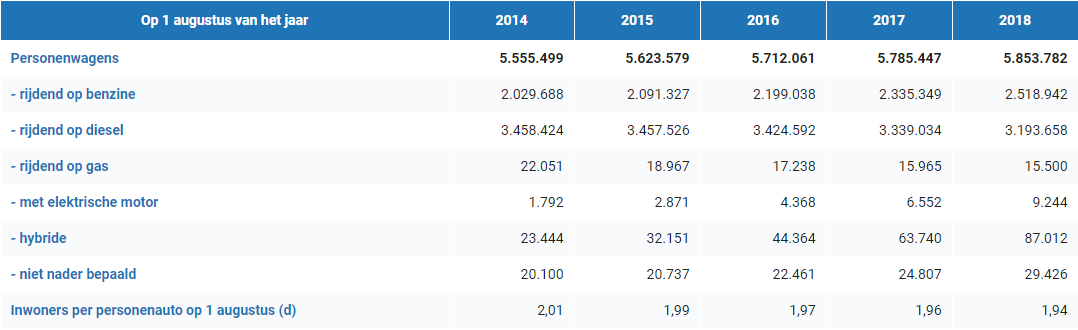
\includegraphics[width=\linewidth]{images/wagenpark_belgie.png}
  \caption{Grootte van het voertuigenpark 2014-2018 (bron: statbel.fgov.be)}
  \label{fig:wagenpark}
\end{figure}


\section{Online machine learning voor geïndividualiseerde cadanscontrole}
Deze thesis werkt verder op het prototype geleverd door IntuEdrive. Zoals reeds aangehaald schakelt de fiets automatisch. De trapcadans wordt hierdoor stabiel gehouden, ook wanneer de fietser harder of zachter trapt. Het doel is om deze instelling te veranderen door de cadans van de e-bike in real time te voorspellen aan de hand van de toestand van de fiets, zodat de trapsnelheid zich aanpast aan de huidige omstandigheden en de individuele gebruiker. Deze implementatie zal ervoor zorgen dat de fietser meer aandacht kan besteden aan de weg, waardoor gevaarlijke situaties kunnen vermeden worden. Om de cadans te personaliseren en dynamisch te maken, zal een machine learning algoritme ontwikkeld worden dat de toestand van de fiets als input binnenkrijgt en hiermee de trapsnelheid berekent. Wanneer de fietser besluit om de cadans manueel aan te passen, interpreteert het algoritme dit als een signaal om bij te leren.
\\\\
Om de performantie van het machine learning algoritme te testen zal het volledig systeem fiets-fietser-cadanscontrole gesimuleerd worden. Het fietsmodel wordt geleverd door IntuEdrive en zal geïmplementeerd worden in python. Vervolgens worden een aantal machine learning algoritmes vergeleken op basis van een aantal vooraf gedefinieerde performance indicatoren. De machine learning algoritmes zijn afkomstig uit scikit-learn, een machine learning library.
\\\\
De cadanscontrole moet aan verschillende eisen voldoen. Het algoritme moet draaien op een Raspberry Pi, samen met het controleprogramma van de fiets. Door deze beperkte resources moet het algoritme zo efficiënt mogelijk zijn. De voorspellingen moeten bijna in real time berekend worden. Het doel is om aan 10Hz de cadans aan te passen, maar hoe meer voorspellingen per seconde, hoe beter. Tragere voorspellingen kunnen hinderlijk zijn voor het rijgedrag. Ten slotte moet er ook rekening gehouden worden met de veiligheid van de fietser. Opeenvolgende voorspellingen mogen niet te veel van elkaar verschillen, anders zou de fietser erdoor gestoord kunnen worden en zijn concentratie verliezen. Bovendien mag de cadans nooit hoger dan een bepaalde maximum limiet ingesteld worden.
\\\\
De algoritmes worden geëvalueerd op basis van de mean squared error tussen de ingestelde cadans - afkomstig van het machine learning algoritme - en de zogenaamde \textit{\gls{fcc}} van de fietser. Die freely chosen cadence is niet precies gekend en wordt in de simulatie bepaald aan de hand van een fietsersmodel. Dit is een functie die de toestand van de fiets en de fietser (rijsnelheid, helling,...) afbeeldt op de trapsnelheid die de fietser in dat geval het meest comfortabel vindt. Simpel gezegd is het fietsersmodel een functie met als input de toestand van de fiets en als output een “optimale cadans”. Deze functie is speculatief en kan makkelijk aangepast worden. Op welke basis de fietser precies zijn freely chosen cadence bepaalt is voor dit onderzoek weinig relevant. Het gaat er hier vooral om dat het machine learning algoritme het fietsersmodel kan achterhalen.
\\
\begin{center}
Fietsersmodel:\tab fcc = f(snelheid,koppel,vermogen,helling,...)
\end{center}
Het algoritme moet kunnen bijleren met een kleine hoeveelheid data. De gebruiker zal immers niet vaak manuele aanpassingen doen aan de cadans. Te veel data gebruiken kan een negatieve invloed hebben op reeds correcte voorspellingen. Het algoritme moet ook snel bijleren. Elke verandering moet zo snel mogelijk doorgevoerd worden en moeten een betekenisvolle impact hebben.
\section{Huidige systeem}
De fiets van intuEdrive gebruikt een e-CVT – een elektrische continu variabele transmissie – die ervoor zorgt dat er naadloos geschakeld kan worden tussen versnellingen, in tegenstelling tot het traditionele ketting-en-tandwiel systeem. Dit oude systeem schakelt in discrete trappen, waardoor de fietser tijdens het schakelen een discontinuïteit voelt. Het CVT-systeem gebruikt 2 motoren en schakelt traploos. Eén van de motoren regelt de trapcadans, de andere motor regelt het ondersteuningsniveau. Het ondersteuningsniveau bepaald hoeveel extra elektrisch vermogen er geleverd wordt, bovenop wat de fietser zelf levert.\vphantom{\gls{cvt}}
\\\\
Figuur \ref{fig:Blokdiagram van het fiets-fietser-controller systeem} toont een blokdiagram van het systeem fiets-fietser-controller. We gaan ervan uit dat de fietser op elk moment een bepaalde referentiesnelheid (\gls{v_ref}) probeert te halen, hier aangeduid met r. Deze kan variëren naar gelang de situatie, maar is voor elke gebruiker anders. Tijdens het fietsen geeft de fietser input aan de fiets. Zo kan hij of zij het geleverde koppel variëren (\gls{t_cy}), i.e. meer of minder kracht op de pedalen zetten of de cadans aanpassen met de knoppen (\gls{u_c}). Inputs en fysische toestand van de fiets worden gemeten door sensoren op de fiets: het koppel (\gls{t_cy,m}), de hoek van de trapas (\gls{theta_cr}), snelheid (\gls{v_bike}), helling (\gls{helling}), etc. $T_{cy}$ en $T_{cy,m}$ zijn niet hetzelfde, want er kunnen fouten gebeuren tijdens het meten. De vector van meetwaarden (\gls{y}) is input voor de fietscontroller. De fietscontroller stuurt de motoren in de E-bike aan op basis van de metingen \gls{y} en de ingestelde referentiecadans. De cadanscontroller die in deze thesis uitgewerkt zal worden zal op basis van dezelfde metingen een gepersonaliseerde referentiecadans (\gls{fcc_est}) voorspellen die als input dient voor de controller.
\tikzset{
block/.style = {draw, fill=white, rectangle, minimum height=3em, minimum width=9em},
tmp/.style  = {coordinate}, 
input/.style = {coordinate},
output/.style= {coordinate},
box/.style={draw=gray,dashed,fill opacity = 0,thick,inner sep=5pt},
test/.style = {}
}
\begin{gather*}
r = \begin{bmatrix}
       v_{ref}  
     \end{bmatrix} \tab
u_{cy} = \begin{bmatrix}
       T_{cy} \\ u_c  
     \end{bmatrix} \tab
u_{contr} = \begin{bmatrix}
       ????  
     \end{bmatrix} \tab
cc = \begin{bmatrix}
       FCC_{est}  
     \end{bmatrix} \tab
y = \begin{bmatrix} 
       \theta _{cr} \\ T_{cy,m} \\ v_{bike} \\ \alpha
     \end{bmatrix} 
\end{gather*}
\begin{figure}[h]
\begin{tikzpicture}[auto, node distance=2cm,>=latex']
    \node [input, name=fietsinput] (fietsinput) {};
    \node [block, right of=fietsinput,node distance=5cm] (fietser) {Fietser};
    \node [tmp, right of=fietser,node distance=3cm] (above_fietser){};
    \node [block, below of=above_fietser,node distance=3cm] (fiets) {Fiets};
    \node [tmp, left = 1.5cm of fiets] (left_fiets) {};
    \node [block, below of=fiets] (controller){Controller};
    \node [tmp, left = 1.5cm of controller] (left_controller) {};
    \node [block, below of=controller] (cadencecontroller) {Cadanscontroller};   
    \node [tmp, left = 1.5cm of cadencecontroller] (left_cadencecontrol) {};
    \node [tmp, right of=fiets,node distance=3cm] (right_fiets){};    
    \node [tmp, right of=right_fiets] (output){};    
    \draw [->] (fietsinput) -- node{$r$} (fietser);
    \draw [->] (fietser) |- (above_fietser) -- node{$u_{cy}$} (fiets);
    \draw [->] (controller.west) |- (left_controller) |- node {$u_{contr}$} (fiets.west);
    \draw [->] (cadencecontroller) -- node{$cc$} (controller);
   	\draw [->] (right_fiets) |- (controller.east);
   	\draw [->] (right_fiets) |- (cadencecontroller.east);
    \draw [->] (fiets) -- node [name=y] {$y$}(output);   
\end{tikzpicture}
\caption{Blokdiagram van het fiets-fietser-controller systeem}
  \label{fig:Blokdiagram van het fiets-fietser-controller systeem}
\end{figure}
\\\\
\chapter{Methode}
\section{De fietssimulatie}
Er wordt een simulatie gemaakt die de toestand van de fiets zo goed mogelijk probeert te benaderen. Er zal geen rekening gehouden worden met het manoeuvreren van de fiets of van tegenwind. Enkel de relevante meetwaarden worden bijgehouden. De simulatie is geparametriseerd om eenvoudig verschillende scenario’s te testen.
\\\\
Het voordeel van de fietssimulatie is de enorme flexibiliteit. Uren aan data kunnen in een moment tijd gegenereerd worden, waardoor het makkelijk is om verschillende tests uit te voeren. Hiervoor moeten slechts enkele instellingen aangepast worden. Het is ook mogelijk om slechts een enkele parameter aan te passen tijdens tests terwijl de rest constant blijft (\textit{ceteris paribus}), wat praktisch onmogelijk is in een veldtest. Omdat de simulatie bovendien een duidelijke referentie genereert voor de FCC (output van het fietsersmodel), kan de performantie van de cadanscontroller op een kwantitatieve manier worden geëvalueerd. Tijdens een veldtest zou de fietser alleen kwalitatief kunnen aangeven of hij of zij de voorspelde cadans goed vind. 
\section{Modelleren van het fietserkoppel}
Het fietserkoppel wordt gemodelleerd als een sinusfunctie met twee pieken per omwenteling van de trapas (2 benen), met het DC koppel van de fietser als parameter.
\\
\begin{align*}
 T_{cy} &= T_{dc}(1+sin(2\theta_{cr}-\frac{\pi}{6}))
\end{align*}
\\
Uit deze formule is het ook meteen duidelijk dat het DC koppel ook het vermogen-equivalent koppel is. Dat wil zeggen dat het DC koppel gedurende een volledige omwenteling van de trapas evenveel arbeid levert als het fietserkoppel.
\\\\
Het gemiddelde koppel geleverd door de fietser wordt gemodelleerd als een proportionele regelaar. Het doel is om een bepaalde snelheid, $v_{ref}$, te behalen. Hoe groter het verschil is tussen de referentie snelheid en de eigenlijke snelheid, hoe meer kracht er geleverd zal worden. Als deze referentie snelheid overschreden wordt, dan zal er geen koppel meer geleverd worden. Dit wordt ook wel freewheelen genoemd. Om de kracht van de actor te limiteren, wordt er een maximum koppel ingesteld naar gelang de huidige cadans (\gls{omega_cr}). Zo wordt er meer kracht geleverd wanneer de cadans laag is, net zoals in de werkelijkheid. \gls{k} bepaalt de agressiviteit van de regelaar. De formules zien er als volgt uit:

\begin{gather*}
T_{dc,max} = \frac{-\omega_{cr}}{2}+60 \tab (Figuur\ \ref{fig:koppeltoerentalkarakteristiek}) \\
T_{dc} = min(T_{dc,max},max(0,-K*(v_{bike}-v_{ref}))
\end{gather*}

\begin{figure}
  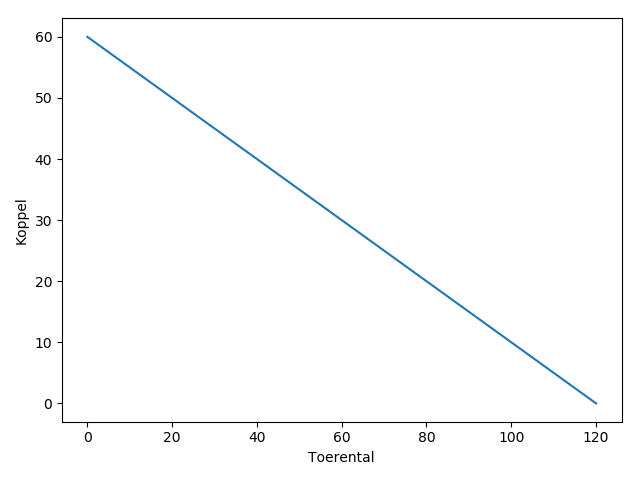
\includegraphics[width=\linewidth]{images/koppel-toerentalkarakteristiek.png}
  \caption{Het koppel-toerentalkarakteristiek}
  \label{fig:koppeltoerentalkarakteristiek}
\end{figure}

Figuren \ref{fig:menselijkkoppelverloop} en \ref{fig:gesimuleerdkoppelverloop} tonen een menselijk koppelverloop en gesimuleerd koppelverloop, gesampled aan 10Hz. Zoals te zien is het gesimuleerde koppel heel consistent. Het menselijk koppel volgt duidelijk een cyclische functie, maar toont vormen van inconsistentie. Merk wel op dat er telkens een afwisseling is van een hoge en een lage piek. Dit wijst op een dominant been. Figuur \ref{fig:gesimuleerde koppel dominant been} toont een gesimuleerd koppelverloop van een fietser met een dominant been.
\\\\
\begin{figure}[t!]
\centering
\begin{subfigure}{.5\textwidth}
  \centering
  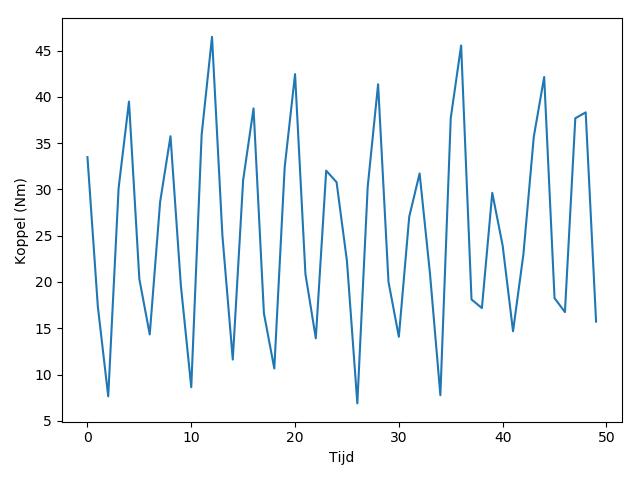
\includegraphics[width=\linewidth]{images/menselijkkoppel.png}
  \caption{Menselijk koppelverloop}
  \label{fig:menselijkkoppelverloop}
\end{subfigure}%
\begin{subfigure}{.5\textwidth}
  \centering
  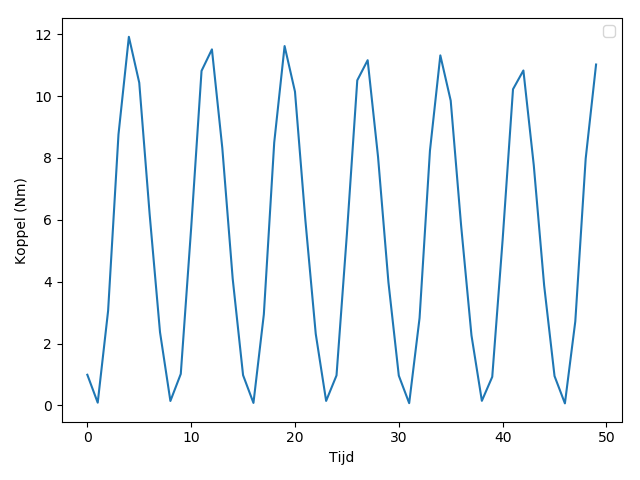
\includegraphics[width=\linewidth]{images/gesimuleerdekoppel.png}
  \caption{Gesimuleerd koppelverloop}
  \label{fig:gesimuleerdkoppelverloop}
\end{subfigure}
\begin{subfigure}{.5\textwidth}
  \centering
  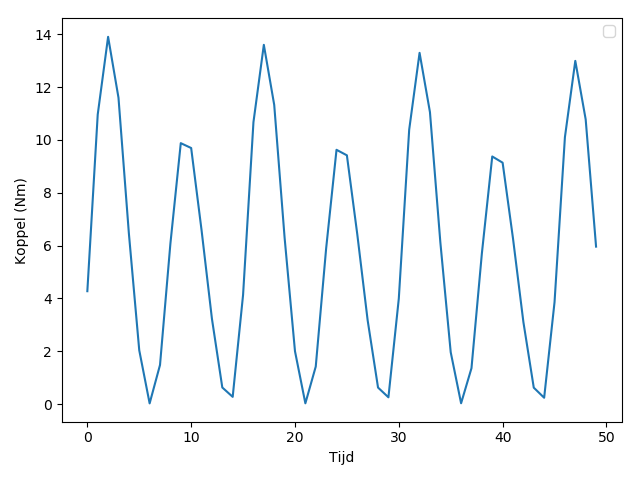
\includegraphics[width=\linewidth]{images/gesimuleerdekoppeldominantbeen.png}
  \caption{Gesimuleerd koppelverloop met dominant been}
  \label{fig:gesimuleerde koppel dominant been}
\end{subfigure}
\caption{Het koppelverloop van een mens (linksboven), de simulatie (rechtsboven) en een gesimuleerd dominant been (onderaan)}
\label{fig:test}
\end{figure}
\newpage
\begin{wrapfigure}{R}{0.5\textwidth}
  \centering
  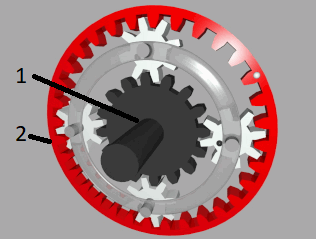
\includegraphics[width=\linewidth]{images/planeetwielmechanisme.png}
  \caption{Planeetwielmechanisme (bron: wikipedia)}
  \label{fig:planeetwielmechanisme}
\end{wrapfigure}

\noindent $T_{cy}$ is het koppel op de trapas. Dit moet nog overgebracht worden op het achterwiel. CoSaR maakt gebruik van een planeetwielmechanisme (figuur \ref{fig:planeetwielmechanisme}). Dit mechanisme laat toe om een grote overbrengingsverhouding te voorzien in een kleine ruimte. Het achterwiel-koppel wordt beïnvloed door het aantal tanden op het zonnewiel (1; \gls{ns}) en het ringwiel (2; \gls{nr}) en de overbrengingsverhouding tussen de trapas en het ringwiel (\gls{k_cr,r}). Het koppel op het achterwiel (\gls{t_rw}) ziet er als volgt uit:
\begin{gather*}
T_{rw}=T_{cy}*k_{cr,r}*\frac{nr+ns}{nr}
\end{gather*}
\\\\
Bovenop het vermogen geproduceerd door de fietser, levert CoSaR extra ondersteuning a.d.h.v. een motor (\gls{t_mg2}) gekoppeld aan het voorwiel. De fietser kan zelf een ondersteuningsniveau (\gls{s}) instellen tussen 0 en 5. Hoe hoger dit ondersteuningsniveau, hoe minder inspanning de fietser moet leveren. 
\begin{gather*}
T_{MG2}=min(35,S\thinspace .\thinspace T_{cy})
\end{gather*}

\section{Het fietsersmodel}
Hoe kiest een fietser zijn cadans? Dit is voor elke fietser verschillend en er is nog nauwelijks onderzoek naar gebeurd. Wielrenners trainen om sneller te kunnen trappen omdat dit efficiënter is.. Ze kunnen een gemiddeld vermogen leveren van 300 Watt. De doorsnee fietser levert gemiddeld ongeveer 75 Watt tijdens een normale fietstocht. Het fietsersmodel zal hierop worden afgesteld, aangezien wielrenners niet de voornaamste doelgroep zijn voor CoSaR.
\\\\
Het fietsersmodel is een functie die op verschillende manieren uitgedrukt kan worden: op basis van de helling, gemiddeld koppel, of een stabiel vermogen. Wat het correcte model is wordt in deze thesis niet uitgewerkt. Het is vooral van belang dat de cadanscontroller het model zo snel en zo nauwkeurig mogelijk kan achterhalen, ongeacht wat het model precies is. Hier wordt de volgende aanname gemaakt: hoe hoger het koppel geleverd door de fietser, hoe hoger de gewenste cadans. Wanneer de fietser bijvoorbeeld een helling oprijdt schakelt hij of zij een versnelling omlaag zodat de kracht die op de pedalen gezet moet worden aangenaam blijft. We stellen hier volgende eenvoudige modellen voor:
\vphantom{\gls{f_k}\gls{f_h}\gls{f_v}}
\begin{align*}
Gemiddeld koppel:\tab fcc &= f_k . T_{dc}\\
Helling:\tab fcc &= f_h . \alpha\\
Snelheid:\tab fcc &= f_v . v_{bike}
\end{align*}
Er wordt verder aangenomen dat de fietser ook een zeker lineariteit verwacht bij lage snelheden. Dat wil zeggen dat een fietser het niet comfortabel vindt wanneer hij of zij snel moet trappen wanneer de fiets nog stilstaat of heel traag rijdt, ook al moet er op dat moment veel koppel geleverd worden om te kunnen vertrekken. Daarom wordt bij lage snelheden de FCC begrensd door een lineair oplopend maximum, te vergelijken met een mechanische fietsversnelling. Omdat de doorsnee fietser niet heel traag of heel snel trapt wordt de FCC begrensd tussen de 40 en 120 rpm. Figuur \ref{fig:cadansverloop} toont een voorbeeld van deze berekening waarbij de fcc is ingesteld op 70 rpm.
\begin{figure}
  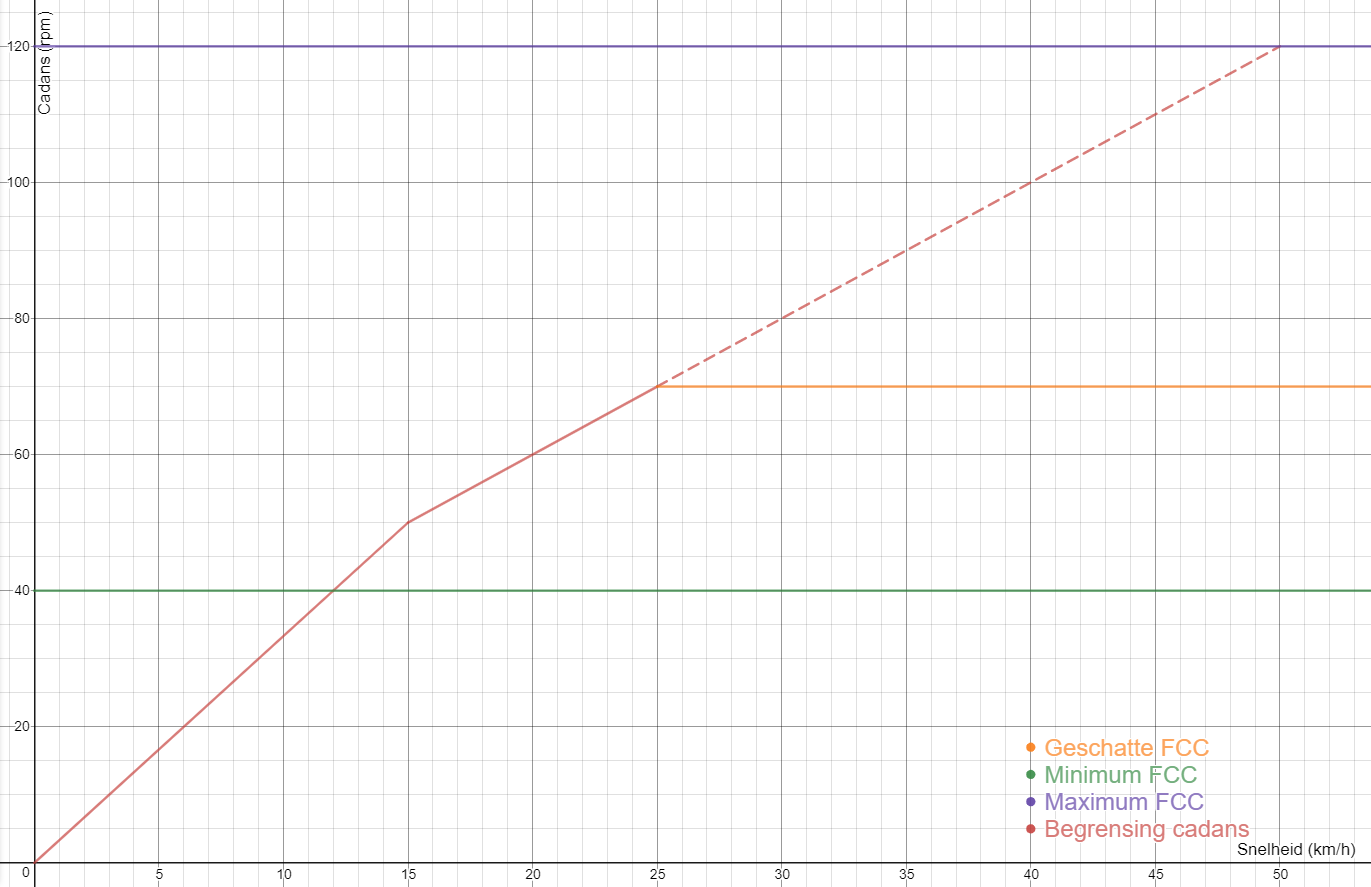
\includegraphics[width=\linewidth]{images/cadansverloop.png}
  \caption{Cadansverloop in functie van de snelheid begrensd door fcc}
  \label{fig:cadansverloop}
\end{figure}
\newpage
\section{Het lastmodel}
De simulatie is voorzien van een lastmodel. Zoals in realiteit, werken lasten in op de fiets. Zwaartekracht, wrijving met de weg en luchtweerstand zijn gemodelleerd als volgt:
\\
\begin{align*}
F_{grav}&=m \ . \ g \ . \ sin \ \alpha \\
F_{friction}&=m \ . \ g. \ c_r \ . \ cos \ \alpha \\
F_{aero}&=\frac{c_d \ . \ \rho_{aero} \ . \ A_{aero} \ . \ v_{bike}^2}{2}
\end{align*}
Samen vormen ze de totale belasting op de fiets, die kwadratisch is in de snelheid.\vphantom{\gls{f_grav}\gls{f_friction}\gls{f_aero}\gls{m}\gls{g}\gls{c_r}\gls{c_d}\gls{rho_aero}\gls{a_aero}\gls{f_load}}
\[F_{load} = F_{grav}+F_{friction}+F_{aero}\]
Deze lasten zorgen ervoor dat de simulatie een realistische hoeveelheid vermogen nodig heeft om een bepaalde snelheid te halen. Er wordt hier geen rekening gehouden met de wind. Ten eerste zou dit extra complexiteit toevoegen aan de simulatie. En ten tweede vermoeden we volgende hypothese:
\\\\
\tab De freely chosen cadence hangt af van de hoeveelheid last, van welke bron dan \tab ook, die de gebruiker ondervindt en de gebruiker zelf.
\\\\
Het voorgestelde lastmodel omvat deze vereiste. Door de helling en referentie snelheid te variëren ondergaat de fietser een veranderende last. Zoals in de realiteit zoeken mensen een bepaalde snelheid te halen. Wanneer de fietser een te hoge last ondervindt, bijvoorbeeld door een berg op te rijden, moet hij of zij meer vermogen genereren om zijn of haar gewenste snelheid te behouden. Hiervoor zijn 2 mogelijkheden: het verhogen van het koppel of de trapsnelheid. Mensen zijn meer geneigd om hun gewenste cadans te behouden, ongeacht het koppel (binnen bepaalde grenzen). De formule voor mechanisch vermogen gaat als volgt:
\[P=T_{cy} \ . \omega_{cr} \]
Om het lastmodel correct te laten werken, moet er nog een helling gegenereerd worden. Om veel werk uit te sparen met het uitstippelen van parcours, wordt dit dynamisch gegenereerd met behulp van perlin noise. Perlin noise kan gebruikt worden om willekeurige getallen te genereren waarbij opeenvolgende getallen weinig van elkaar verschillen. Een perfecte kandidaat dus om terrein te simuleren. Om verschillende trajecten te creëren, kan de seed variabele aangepast worden. Een hellingsgraad wordt in de fietswereld vaak percentueel voorgesteld. Deze implementatie heeft echter radialen nodig. De helling zal beperkt worden tussen $\approx$ 0 en 10\% (0 en 0.1 radialen). Ter vergelijking, de Koppenberg heeft een gemiddeld stijgingspercentage van 11.6\%. Het minimum stijgingspercentage is zo gekozen dat de simulatie zo weinig mogelijk gaat freewheelen.
\begin{figure}[b!]
  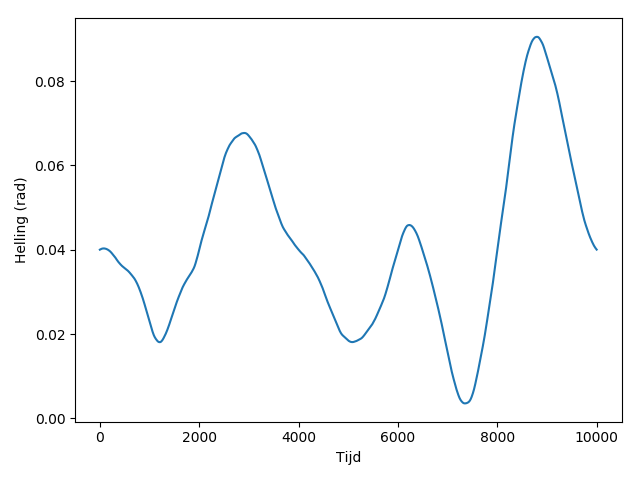
\includegraphics[width=\linewidth]{images/parcour_slope_example.png}
  \caption{Voorbeeld helling verloop}
  \label{fig:hellingverloop}
\end{figure}
\section{Snelheidsvergelijking}
\noindent De snelheid wordt berekend met een standaardformule: vorige snelheid plus acceleratie met respect tot de genomen tijdsprong. De acceleratie is in functie van de last, het totaalgewicht (m), het vermogen geleverd door de fietser op het achterwiel ($T_{rw}$) en het vermogen van een motor bevestigd op het voorwiel ($T_{MG2}$). 
\\\\
De bewegingsvergelijking van de fiets is, met inbegrip van het lastmodel en het fietsersmodel:
\[F \ = \  m \ . \ a \]
Deze vergelijking wordt elke tijdsstap geïntegreerd met behulp van een voorwaartse Euler methode:
\[v_{bike}[h] \ = \ v_{bike}[h-1] \ + \Delta t  \ . \frac{1}{m} \ . \ (\frac{T_{MG2} \ + \ T_{rw}}{r_w} \ - \ F_{load})\]
De volledige simulatie ziet er als volgt uit:
\\\\
 \fbox{\begin{minipage}{\linewidth}
for h in 1..$\#$tijdssprongen\\
\tab $T_{dc,max} = \frac{-\omega_{cr}[h-1]}{2}+60$\\
\tab $T_{dc} = min(T_{dc,max}, \ max(0,-K*(v_{bike}[h-1]-v_{ref}))$\\
\tab $fcc = f(T_{dc})$\\
\tab $\omega_{cr}=cadans(v_{bike}[h-1], \ T_{dc}, \ fcc)$\\
\tab $\theta_{cr}=\theta_{cr}[h-1] + \Delta t \ . \ \omega_{cr}$ \\
\tab $T_{cy} = T_{dc}(1+sin(2\theta_{cr}-\frac{\pi}{6}))$\\
\tab $T_{rw}=T_{cy}*k_{cr,r}*\frac{nr+ns}{nr}$\\
\tab $T_{MG2}=min(35, \ S \ . \ T_{cy})$\\
\tab $F_{grav}=m \ . \ g \ . \ sin \ \alpha$\\
\tab $F_{friction}=m \ . \ g. \ c_r \ . \ cos \ \alpha$\\
\tab $F_{aero}=\frac{c_d \ . \ \rho_{aero} \ . \ A_{aero} \ . \ v_{bike}[h-1]^2}{2}$\\
\tab $F_{load} = F_{grav}+F_{friction}+F_{aero}$\\
\tab $v_{bike} \ = \ v_{bike}[h-1] \ + \Delta t  \ . \frac{1}{m} \ . \ (\frac{T_{MG2} \ + \ T_{rw}}{r_w} \ - \ F_{load})$
\end{minipage}}
\chapter{Resultaten}
\chapter{Discussie}





\newpage
% ----------------------- Achterblad ------------------------------
% Vergeet niet de tekst aan te passen:
% - Afdeling
% - Adres van de afdeling
% - Telefoon en faxnummer
% -----------------------------------------------------------------
\thispagestyle{empty}
\sffamily
%
\begin{textblock}{191}(113,-11)
{\color{blueline}\rule{160pt}{5.5pt}}
\end{textblock}
%
\begin{textblock}{191}(168,-11)
{\color{blueline}\rule{5.5pt}{59pt}}
\end{textblock}
%
\begin{textblock}{183}(-24,-11)
\textblockcolour{}
\flushright
\fontsize{7}{7.5}\selectfont
\textbf{Computerwetenschappen}\\
Celestijnenlaan 200 A bus 2402\\
3000 LEUVEN, BELGI\"{E}\\
tel. + 32 16 32 77 00\\
fax + 32 16 32 79 96\\
www.kuleuven.be\\
\end{textblock}
%
\begin{textblock}{191}(154,-7)
\textblockcolour{}
\includegraphics*[height=16.5truemm]{sedes}
\end{textblock}
%
\begin{textblock}{191}(-20,235)
{\color{bluetitle}\rule{544pt}{55pt}}
\end{textblock}
\end{document}
